\section{Introduction}
\IEEEPARstart{R}{apid} detection and mapping of slope failures following natural disasters such as earthquakes, typhoons, and torrential rainfall are crucial for emergency disaster response and search-and-rescue operations~\cite{meena2023hrgldd}. Landslides sever critical transportation networks, dam river valleys, and bury mountain communities, requiring first responders to make urgent triage decisions. In the immediate aftermath of widespread geohazards, satellite remote sensing provides the primary observation modality to assess inaccessible terrain across hundreds of square kilometers~\cite{meena2023hrgldd}.

The availability of daily, high-resolution constellation imaging—most notably PlanetScope satellites providing four-band multispectral imagery (Blue, Green, Red, Near-Infrared) at 3~m ground sampling distance (GSD)—has made regional post-disaster monitoring operational~\cite{meena2023hrgldd}. However, automated extraction of landslides from high-resolution optical imagery remains challenging. Fresh slope failures in vegetated mountain terrain are physical events: the vegetative canopy is sheared away by the mass movement, exposing bare soil, fractured rock scarps, and transported debris. While this displacement causes an abrupt drop in vegetative reflection, non-landslide landscape features—including agricultural terraces, dry river gravel, dirt roads, and deforestation patches—exhibit nearly identical low-vegetation signatures~\cite{meena2023hrgldd,sghnet2026}. Furthermore, severe topographic hill-shadows in steep valleys compress radiance values, confounding automated classifiers.

Recent literature has deployed deep convolutional neural networks, such as U-Net~\cite{ronneberger2015unet} and Deep Residual U-Net (ResU-Net)~\cite{zhang2018resunet}, to benchmark datasets including the High-Resolution Global Landslide Detector Database (HR-GLDD)~\cite{meena2023hrgldd}. While baseline deep architectures improve over pixel-based thresholds, they treat multispectral channels as arbitrary, independent feature planes. By convolving spectral bands uniformly without explicitly incorporating the non-linear biophysical ratios that govern vegetation health, standard networks frequently produce extensive false-positive clusters along riverbeds and cultivated clearings~\cite{meena2023hrgldd}. Recently, DCA-UNet (Song et al., 2026~\cite{dcaunet2026}) demonstrated that combining deformable convolutions with aggregated attention achieves $74.41\%$ F1 on HR-GLDD; however, it requires 29.50~million parameters and heavy runtime memory. Similarly, SGH-Net~\cite{sghnet2026} explored spectrally guided attention for multimodal optical and digital elevation model (DEM) fusion, but depends on auxiliary topographic layers that are often unavailable in rapid-response pipelines.

\begin{figure}[t]
\centering
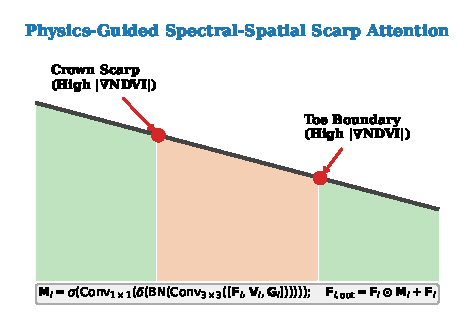
\includegraphics[width=\columnwidth]{figures/fig_scattering_mechanism.pdf}
\caption{Schematic of the physical scarp contrast principle. Fresh slope failures shear vegetative canopy, creating steep localized gradients in Normalized Difference Vegetation Index ($|\nabla \text{NDVI}|$). S$^3$-Net couples these biophysical gradients directly into residual spatial attention gates to delineate subtle scarp geometry and enhance boundary recall.}
\label{fig:mechanism}
\end{figure}

To address these operational limitations, we introduce the Spectral-Spatial Scarp Network (S$^3$-Net), an ultra-lightweight (2.11M parameters, $\approx 14\times$ smaller than DCA-UNet), physics-guided architecture tailored for rapid satellite mapping (Fig.~\ref{fig:mechanism}). S$^3$-Net explicitly computes the Normalized Difference Vegetation Index (NDVI) and its spatial gradient magnitude $|\nabla \text{NDVI}|$, injecting these physical scarp indicators directly into multi-scale residual spatial attention modules along the encoder-decoder skip connections. By gating deep spatial features with physical vegetation scarp contrast, the network recovers subtle slip boundaries without requiring external DEM downloads.

We evaluate S$^3$-Net on the official, globally distributed HR-GLDD benchmark across 1,758 real PlanetScope satellite patches spanning 10 global disaster events across South Asia, East Asia, Southeast Asia, Oceania, and Latin America~\cite{meena2023hrgldd}. Across three independent random seeds, S$^3$-Net achieves a pooled micro F1-score of $70.18\% \pm 0.25\%$, an IoU of $54.06\% \pm 0.29\%$, and a per-tile macro F1 of $58.52\% \pm 0.24\%$ on the official held-out test split. True tile-level cluster-bootstrap tests over the 355 independent test tiles, pooling all three seeds, confirm statistically significant macro F1 improvements of $+3.69\%$ ($p < 0.001$) over standard U-Net, $+0.60\%$ ($p = 0.005$) over ResU-Net, and $+1.44\%$ ($p < 0.001$) over a capacity-matched unguided attention ablation. Benchmarking yields a throughput of 462.6~tiles/s (2.16~ms/tile), establishing a practical, deployable balance between accuracy, parameter efficiency, and scarp boundary delineation.
